\documentclass{standalone}
\usepackage{tikz}

\begin{document}

\tikzset{every picture/.style={line width=0.75pt}} %set default line width to 0.75pt

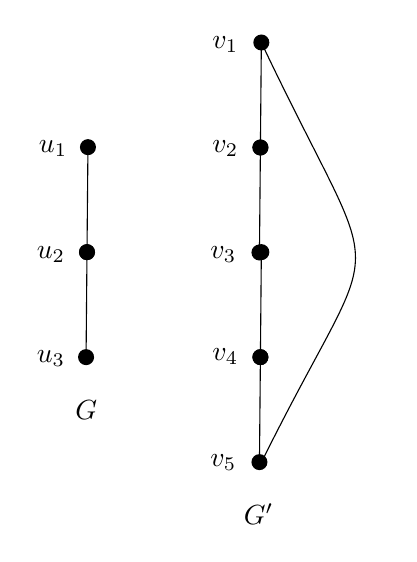
\begin{tikzpicture}[x=0.75pt,y=0.75pt,yscale=-1,xscale=1]
%uncomment if require: \path (0,300); %set diagram left start at 0, and has height of 300

%Straight Lines
\draw    (238.33,40.83) -- (237.88,91.42) ;
\draw [shift={(237.88,91.42)}, rotate = 90.52] [color={rgb, 255:red, 0; green, 0; blue, 0 }  ][fill={rgb, 255:red, 0; green, 0; blue, 0 }  ][line width=0.75]      (0, 0) circle [x radius= 3.35, y radius= 3.35]   ;
\draw [shift={(238.33,40.83)}, rotate = 90.52] [color={rgb, 255:red, 0; green, 0; blue, 0 }  ][fill={rgb, 255:red, 0; green, 0; blue, 0 }  ][line width=0.75]      (0, 0) circle [x radius= 3.35, y radius= 3.35]   ;
%Straight Lines
\draw    (237.88,91.42) -- (237.42,142) ;
\draw [shift={(237.42,142)}, rotate = 90.52] [color={rgb, 255:red, 0; green, 0; blue, 0 }  ][fill={rgb, 255:red, 0; green, 0; blue, 0 }  ][line width=0.75]      (0, 0) circle [x radius= 3.35, y radius= 3.35]   ;
\draw [shift={(237.88,91.42)}, rotate = 90.52] [color={rgb, 255:red, 0; green, 0; blue, 0 }  ][fill={rgb, 255:red, 0; green, 0; blue, 0 }  ][line width=0.75]      (0, 0) circle [x radius= 3.35, y radius= 3.35]   ;
%Straight Lines
\draw    (238.33,141.83) -- (237.88,192.42) ;
\draw [shift={(237.88,192.42)}, rotate = 90.52] [color={rgb, 255:red, 0; green, 0; blue, 0 }  ][fill={rgb, 255:red, 0; green, 0; blue, 0 }  ][line width=0.75]      (0, 0) circle [x radius= 3.35, y radius= 3.35]   ;
\draw [shift={(238.33,141.83)}, rotate = 90.52] [color={rgb, 255:red, 0; green, 0; blue, 0 }  ][fill={rgb, 255:red, 0; green, 0; blue, 0 }  ][line width=0.75]      (0, 0) circle [x radius= 3.35, y radius= 3.35]   ;
%Straight Lines
\draw    (237.88,192.42) -- (237.42,243) ;
\draw [shift={(237.42,243)}, rotate = 90.52] [color={rgb, 255:red, 0; green, 0; blue, 0 }  ][fill={rgb, 255:red, 0; green, 0; blue, 0 }  ][line width=0.75]      (0, 0) circle [x radius= 3.35, y radius= 3.35]   ;
\draw [shift={(237.88,192.42)}, rotate = 90.52] [color={rgb, 255:red, 0; green, 0; blue, 0 }  ][fill={rgb, 255:red, 0; green, 0; blue, 0 }  ][line width=0.75]      (0, 0) circle [x radius= 3.35, y radius= 3.35]   ;
%Straight Lines
\draw    (154.33,141.83) -- (153.88,192.42) ;
\draw [shift={(153.88,192.42)}, rotate = 90.52] [color={rgb, 255:red, 0; green, 0; blue, 0 }  ][fill={rgb, 255:red, 0; green, 0; blue, 0 }  ][line width=0.75]      (0, 0) circle [x radius= 3.35, y radius= 3.35]   ;
\draw [shift={(154.33,141.83)}, rotate = 90.52] [color={rgb, 255:red, 0; green, 0; blue, 0 }  ][fill={rgb, 255:red, 0; green, 0; blue, 0 }  ][line width=0.75]      (0, 0) circle [x radius= 3.35, y radius= 3.35]   ;
%Straight Lines
\draw    (154.79,91.25) -- (154.33,141.83) ;
\draw [shift={(154.33,141.83)}, rotate = 90.52] [color={rgb, 255:red, 0; green, 0; blue, 0 }  ][fill={rgb, 255:red, 0; green, 0; blue, 0 }  ][line width=0.75]      (0, 0) circle [x radius= 3.35, y radius= 3.35]   ;
\draw [shift={(154.79,91.25)}, rotate = 90.52] [color={rgb, 255:red, 0; green, 0; blue, 0 }  ][fill={rgb, 255:red, 0; green, 0; blue, 0 }  ][line width=0.75]      (0, 0) circle [x radius= 3.35, y radius= 3.35]   ;
%Curve Lines
\draw    (238.33,40.83) .. controls (299.28,169.42) and (298.28,121.92) .. (238.42,243) ;



% Text Node
\draw (138,92) node   {$u_{1}$};
% Text Node
\draw (137,143) node   {$u_{2}$};
% Text Node
\draw (137,193) node   {$u_{3}$};
% Text Node
\draw (221,42) node   {$v_{1}$};
% Text Node
\draw (221,92) node   {$v_{2}$};
% Text Node
\draw (220,143) node   {$v_{3}$};
% Text Node
\draw (221,192) node   {$v_{4}$};
% Text Node
\draw (220,243) node   {$v_{5}$};

% Text Node
\draw (154,218) node   {$G$};
% Text Node
\draw (237,268) node   {$G'$};

\end{tikzpicture}
\end{document}
